\documentclass[preview]{standalone}

\usepackage{amsmath}
\usepackage{amssymb}
\usepackage{stellar}
\usepackage{definitions}
\usepackage{bettelini}
\usepackage{tikz}

\begin{document}

\id{green-gauss-applications}
\genpage

\section{Areas from Green--Gauss}

\begin{snippetdefinition}{plane-domain-area-definition}{Area of a plane domain}
    Let \(\Gamma\) be a positively oriented Jordan curve bounding a bounded
    domain \(\Omega\subseteq\realnumbers^2\). Its area is
    \[
        \operatorname{Area}(\Omega)=\iint_\Omega1\,dx\,dy.
    \]
\end{snippetdefinition}

\begin{snippetproposition}{green-gauss-area-line-integral-formula}{Area as a line integral}
    Under the preceding hypotheses,
    \[
        \operatorname{Area}(\Omega)
        =\frac12\int_{\partial^+\Omega}x\,dy-y\,dx.
    \]
\end{snippetproposition}

\begin{snippetproof}{green-gauss-area-line-integral-formula-proof}{green-gauss-area-line-integral-formula}{Area as a line integral}
    In Green--Gauss, choose
    \(P(x,y)=-y/2\) and \(Q(x,y)=x/2\). Then
    \(Q_x-P_y=1\), and the claimed identity follows.
\end{snippetproof}

\begin{snippetexample}{ellipse-area-green-gauss-example}{Area of an ellipse}
    Compute the area bounded by
    \[
        \frac{x^2}{a^2}+\frac{y^2}{b^2}=1.
    \]
\end{snippetexample}

\begin{snippetsolution}{ellipse-area-green-gauss-solution}{Area of an ellipse}
    Parametrize the boundary positively by
    \(\gamma(t)=(a\cos t,b\sin t)\), \(0\leq t\leq2\pi\). Then
    \begin{align*}
        \operatorname{Area}(\Omega)
        &=\frac12\int_{\partial^+\Omega}x\,dy-y\,dx\\
        &=\frac{ab}{2}\integral[0][2\pi]
        [\cos^2t+\sin^2t][t]\\
        &=\pi ab.
    \end{align*}
\end{snippetsolution}

\begin{snippetproposition}{polar-curve-area-formula}{Area in polar coordinates}
    Let a positively oriented simple closed curve be parametrized by
    \[
        \gamma(\theta)=
        (\rho(\theta)\cos\theta,\rho(\theta)\sin\theta),
        \qquad \theta_1\leq\theta\leq\theta_2.
    \]
    Then the enclosed area is
    \[
        \operatorname{Area}(\Omega)
        =\frac12\integral[\theta_1][\theta_2]
        [\rho(\theta)^2][\theta].
    \]
\end{snippetproposition}

\begin{snippetproof}{polar-curve-area-formula-proof}{polar-curve-area-formula}{Area in polar coordinates}
    With \(x=\rho\cos\theta\) and \(y=\rho\sin\theta\),
    \begin{align*}
        x\,dy-y\,dx
        &=\rho\cos\theta(\rho'\sin\theta+\rho\cos\theta)d\theta\\
        &\quad-\rho\sin\theta(\rho'\cos\theta-\rho\sin\theta)d\theta\\
        &=\rho^2\,d\theta.
    \end{align*}
    Substitute this into the Green--Gauss area formula.
\end{snippetproof}

\begin{snippetexample}{cardioid-area-example}{Area enclosed by a polar curve}
    Compute the area enclosed by
    \[
        \rho=1+\cos\theta,
        \qquad 0\leq\theta\leq2\pi.
    \]
\end{snippetexample}

\begin{snippetsolution}{cardioid-area-solution}{Area enclosed by a polar curve}
    By the polar area formula,
    \begin{align*}
        \operatorname{Area}(\Omega)
        &=\frac12\integral[0][2\pi][(1+\cos\theta)^2][\theta]\\
        &=\frac12\integral[0][2\pi]
        [1+2\cos\theta+\cos^2\theta][\theta]\\
        &=\frac{3\pi}{2}.
    \end{align*}

    \begin{center}
        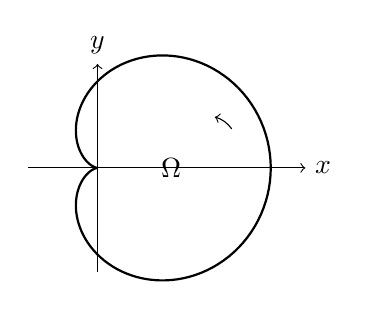
\begin{tikzpicture}[scale=1.1]
            \draw[->] (-0.8,0) -- (2.4,0) node[right] {\(x\)};
            \draw[->] (0,-1.2) -- (0,1.2) node[above] {\(y\)};
            \draw[thick,domain=0:360,samples=160,variable=\t] plot ({(1+cos(\t))*cos(\t)},{(1+cos(\t))*sin(\t)});
            \draw[->] (1.55,0.45) arc[start angle=35,end angle=75,radius=0.35];
            \node at (0.85,0) {\(\Omega\)};
        \end{tikzpicture}
    \end{center}
\end{snippetsolution}

\end{document}
